\documentclass{ximera}
%% handout
%% nohints
%% space
%% newpage
%% numbers


\prerequisites{none}

\title{1.2The Notion of a Limit}

\begin{document}
\begin{abstract}
Limits are a powerful tool.
\end{abstract}
\maketitle

\section{Overview}

In this section we introduce the all-important concept of the \emph{limit}. A limit is a process that we apply to an existing function where we let the input to the function get closer and closer to --- but not become exactly equal to --- a certain input and observe what the outputs do. This process is central for computing instantaneous velocities, and it will lead us to the main concepts of calculus. For now, we will define the concept of the limit and calculate limits using graphical and numerical methods.


\section{Basic learning objectives}

These are the tasks you should be able to perform with reasonable fluency \textbf{when you arrive at our next class meeting}. Important new vocabulary words are indicated \emph{in italics}. 

\begin{itemize}
	\item State the definition of what it means for a function $f$ to have a limit $L$ as $x$ approaches a number $a$, and explain what the definition means in nontechnical terms. 
	\item Calculate limits of functions (or determine if a function fails to have a limit) by examining a graph of the function (see Example 1.1).
	\item Calculate limits of functions (or determine if a function fails to have a limit) by constructing a table of values for the function (see Example 1.2).
\end{itemize}

\section{Advanced learning objectives}

In addition to mastering the basic objectives, here are the tasks you should be able to perform \textbf{after class, with practice}: 

\begin{itemize}
	\item Find the instantaneous velocity of a moving object at a particular point by using limits and the average velocity formulas.
\end{itemize}

\section{Resources}

\noindent
\emph{Reading}: Read Section 1.2, pages 10--17 in Active Calculus 

\noindent
\emph{Watching}: Here are some additional resources that have been developed to support your learning: 

\begin{itemize}
	\item Screencast 1.2.1: \youtube{http://gvsu.edu/s/qm} 
	\item Screencast 1.2.2: \youtube{http://gvsu.edu/s/qn}
	\item Screencast 1.2.3: \youtube{http://gvsu.edu/s/qo}
	\item Screencast 1.2.4: \youtube{http://gvsu.edu/s/qp}
\end{itemize}

\subsection*{Questions}

\noindent Complete each question below.  

\begin{question}
Suppose that $g$ is the function given by the graph below.  Use the graph to answer each of the following questions.

Determine the values $g(-2)$, $g(-1)$, $g(0)$, $g(1)$, and $g(2)$, if defined.  If the function value is not defined, explain what feature of the graph tells you this.
\begin{solution}
\begin{hint}
What are the $y$-values associated with each $x$-value?
\end{hint}
\begin{freeResponse}
$g(-2)=...$
\end{freeResponse}
\end{solution} 

For each of the values $a = -1$, $a = 0$, and $a = 2$, complete the following sentence: ``As $x$ gets closer and closer (but not equal) to $a$, $g(x)$ gets as close as we want to \underline{\hspace{0.3in}}.''
\begin{solution}
\begin{freeResponse}
%
\end{freeResponse}
\end{solution} 

What is the value of $\lim_{x\to1}g(x)=3$?
\begin{multipleChoice}
\choice[correct]{$\lim_{x\to1}g(x)$ does not exist.}
\choice{$\lim_{x\to1}g(x)=3$}
\choice{$\lim_{x\to1}g(x)=2$}
\end{multipleChoice}
\begin{solution}
\begin{hint}
What happens as $x$ gets closer and closer (but not equal) to $a = 1$?  Does the function $g(x)$ get as close as we would like to a single value?
\end{hint}
\end{solution} 

\begin{figure}[h]
\begin{center}
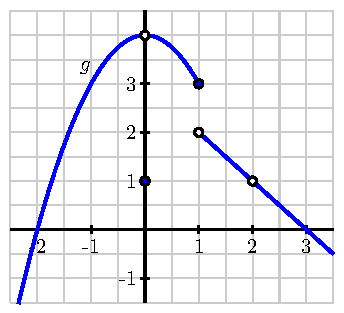
\includegraphics{figures/1_2_PA1.pdf} 
\caption{Graph of $y = g(x)$} \label{F:1.2.PA1}
\end{center}
\end{figure}

\end{question}

\begin{question}
Let $s(t) = 3t - 2$ be the position of a moving object at time $t$.  Find the average velocity of the object on the interval $[3,5]$ (ignoring units).
AV$_{[3,5]}=$ \answer{3} 

Let $s(t) = 3t - 2$ be the position of a moving object at time $t$.  Find a simplified expression for the average velocity of the object on the interval $[3,3+h]$
 (ignoring units).
AV$_{[3,5]}=$ \answer{3} 
\end{question}




\end{document}